\chapter{Elementary Stochastic Processes}

\begin{definition}[Stochastic Processes]
    A stochastic process is a mathematical model of a probabilistic experiment that evolves in time and generates a sequence of numerical values.
\end{definition}

\begin{figure}[H]
    \centering
    \resizebox{!}{0.3\linewidth}
    {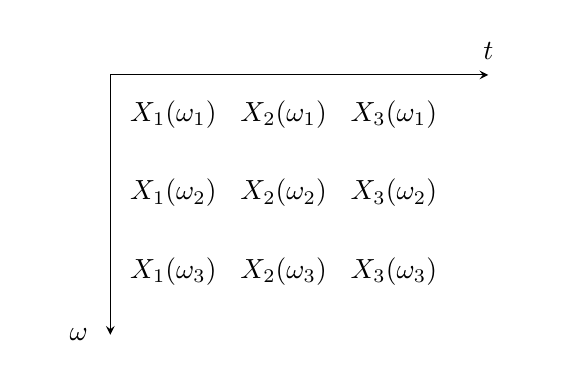
\begin{tikzpicture}[scale = 0.20]
    \definecolor{FFFFFF}{RGB}{255,255,255}
    \draw [draw=none] (37.0,-25.0) rectangle node(IDOL_J-3)[align = center, text width = 1.3 cm,inner sep=0] {$t$} (43.0,-28.0);
    \draw [draw=none] (11.0,-43.0) rectangle node(IDOL_J-4)[align = center, text width = 1.3 cm,inner sep=0] {$\omega$} (17.0,-46.0);
    \draw [draw=none] (17.0,-29.0) rectangle node(IDOL_J-5)[align = center, text width = 1.3 cm,inner sep=0] {$X_1(\omega_1)$} (23.0,-32.0);
    \draw [draw=none] (17.0,-34.0) rectangle node(IDOL_J-6)[align = center, text width = 1.3 cm,inner sep=0] {$X_1(\omega_2)$} (23.0,-37.0);
    \draw [draw=none] (17.0,-39.0) rectangle node(IDOL_J-7)[align = center, text width = 1.3 cm,inner sep=0] {$X_1(\omega_3)$} (23.0,-42.0);
    \draw [draw=none] (24.0,-29.0) rectangle node(ID_J-10)[align = center, text width = 1.3 cm,inner sep=0] {$X_2(\omega_1)$} (30.0,-32.0);
    \draw [draw=none] (24.0,-39.0) rectangle node(ID_J-12)[align = center, text width = 1.3 cm,inner sep=0] {$X_2(\omega_3)$} (30.0,-42.0);
    \draw [draw=none] (31.0,-29.0) rectangle node(ID_J-13)[align = center, text width = 1.3 cm,inner sep=0] {$X_3(\omega_1)$} (37.0,-32.0);
    \draw [draw=none] (31.0,-34.0) rectangle node(ID_J-14)[align = center, text width = 1.3 cm,inner sep=0] {$X_3(\omega_2)$} (37.0,-37.0);
    \draw [draw=none] (31.0,-39.0) rectangle node(ID_J-15)[align = center, text width = 1.3 cm,inner sep=0] {$X_3(\omega_3)$} (37.0,-42.0);
    \draw [draw=none] (24.0,-34.0) rectangle node(ID_J-23)[align = center, text width = 1.3 cm,inner sep=0] {$X_2(\omega_2)$} (30.0,-37.0);
    \draw [-stealth,solid](16.0,-28.0)--(40.0,-28.0);
    \draw [-stealth,solid] (16.0,-28.0) -- (16.0,-44.5);
\end{tikzpicture}
}
    \caption{A Sample Space for a Stochastic Process}
\end{figure}

\begin{remark}
    \textbf{In the following two process, it is essential to distinguish ``measure by time'' and ``measure by successes'', e.g., given a number of successes, how long does it take to achieve them, or given a time interval, how many successes are achieved.}
\end{remark}

\section{Bernoulli Process}

\subsection{Definition and Properties}
\begin{definition}[Bernoulli Process]
    Bernoulli process is a sequence $X_1, X_2, \ldots$ of i.i.d. Bernoulli RVs $X_i$ with
    \begin{equation}
    \begin{aligned}
        \mathbf{P}(\text{success}) &= \mathbf{P}(X_i = 1) = p \\ 
        \mathbf{P}(\text{failure}) &= \mathbf{P}(X_i = 0) = 1 - p 
    \end{aligned}
    \end{equation}
    for each $i$.
\end{definition}
\begin{example}[Examples of Bernoulli Process]
    \begin{itemize}
        \item Sequence of lottery wins/losses
        \item Sequence of transistor qualified/unqualified
        \item Arrivals (each second) to a bank
        \item Arrivals (at each time slot) to server
    \end{itemize}
\end{example}
\begin{property}[Property of Bernoulli Process]
    \begin{itemize}
        \item \textbf{Independence:} For any given time $n$, the sequence of $X_{n+1}, X_{n+2}, \ldots$ is also a Bernoulli process, and is independent from $X_1, \ldots , X_n$.
        \item \textbf{Memoryless:}  Let $n$ be a given time and let $\overline{T}$ be the time of the first success after time $n$. Then $\overline{T} - n$ has a geometric distribution with parameter $p$, and is independent of the RVs $X_1, \ldots X_n$.
    \end{itemize}
\end{property}
\begin{proof}
    Let $\overline{T}$ be the first time after $n$ that $X_i = 1$. Then, the probability that $\overline{T} - n$, conditioning $n$, is given by
    \begin{equation}
        \mathbf{P}(\overline{T} - n = t \mid n) = \mathbf{P}(X_{n+1} = 0, X_{n+2} = 0, \ldots, X_{n+t-1} = 0, X_{n+t} = 1) = p(1-p)^{t-1} = \mathbf{P}(t)
    \end{equation}
\end{proof}

\begin{example}[Example of Memoryless Property]
    Let $N$ be the first $i$ for which $X_{i-1} = X_i = 1$. What is the probability $\mathbf{P}\qty(X_{N+1} = X_{N+2} = 0)$ that there are no successes in the two trials that follow?
\end{example}
\begin{solution}
    Use total probability theorem and memoryless property
    \begin{equation}
    \begin{aligned}
        \mathbf{P}(X_{N+1} = X_{N+2} = 0) &= \sum_{n=1}^{\infty} \mathbf{P}(X_{N+1} = X_{N+2} = 0 \mid N = n) \cdot \mathbf{P}(N = n) \\ 
        &= (1 - p)^2 \sum_{n=1}^{\infty} \mathbf{P}(N = n) = (1 - p)^2
    \end{aligned}
    \end{equation}
\end{solution}

\subsection{Interarrival Times}
Denote the time of the $k$-th success as $Y_k$, and the $k$-th interarrival time as $T_k$, that is 
\begin{equation}
    T_1 = Y_1, \quad T_k = Y_k - Y_{k-1}, \quad Y_k = T_1 + T_2 + \ldots + T_k
\end{equation}
According to the memoryless property, the interarrival times $T_k$ are i.i.d. geometric RVs with parameter $p$, which yields an alternative description of the Bernoulli process.
\begin{definition}[Alternative Description of the Bernoulli Process]
    \begin{enumerate}
        \item Start with a sequence of i.i.d. geometric RVs $T_1, T_2, \ldots$ with parameter $p$, and let these stand for the interarrival times.
        \item Record a success $X_i = 1$ at times $i = Y_k = T_1 + T_2 + \ldots + T_k$, otherwise record a failure $X_i = 0$.
        \item The sequence $X_i$ is then a Bernoulli process with parameter $p$.
    \end{enumerate}
\end{definition}

Also, we can measure the expectation and variance of the time until the $k$-th success, which is given by
\begin{align}
    \E\qty[Y_k] &= \sum_{i=1}^{k} \E\qty[T_i] = \frac{k}{p} \\
    \var\qty(Y_k) &= \sum_{i=1}^{k} \var\qty(T_i) = \frac{k(1-p)}{p^2}
\end{align}
Detailedly, the distribution of $Y_k$ is given by
\begin{equation}
    p_{Y_k}(t) = \binom{t-1}{k-1} p^k (1-p)^{t-k}
\end{equation}
meaning that the time until the $k$-th success is distributed as a negative binomial distribution with parameters $k$ and $p$, which can be proved as follows:
\begin{proof}
    For $t \geq k$, we observe that the event $\{Y_k = t\}$ will occur if and only if both of the following two events $A$ and $B$ occur:
    \begin{itemize}
        \item Event $A$: there is a success at time $t$.
        \item Event $B$: there are exactly $k-1$ successes in the first $t-1$ trials.
    \end{itemize}
    The probability of event $A$ and event $B$ is given by
    \begin{equation}
        \mathbf{P}(A) = p, \quad \mathbf{P}(B) = \binom{t-1}{k-1} p^{k-1} (1-p)^{t-k}
    \end{equation}
    Since $A$ and $B$ are independent, we have
    \begin{equation}
        \mathbf{P}(Y_k = t) = \mathbf{P}(A) \cdot \mathbf{P}(B) = \binom{t-1}{k-1} p^k (1-p)^{t-k}
    \end{equation}
\end{proof}

\subsection{Splitting and Merging}
For a Bernoulli process with parameter $p$, whenever there is a success, we can split success into process $A$ or process $B$ (mutually exclusively) with probabilities $p_A$ and $p_B$, respectively, where $p_A + p_B = 1$; whenever there is a failure, we record it as a failure in both processes. The resulting processes $A$ and $B$ are also Bernoulli processes with parameters $p\cdot p_A$ and $p \cdot p_B$, respectively. The proof is obvious. \textbf{Non of the three processes are independent point-wise, but the two resulting processes $A$ and $B$ are independent as a whole. (Futher studying in course ``Probability and Stochastic Processes (2)'')}
\begin{figure}[H]
    \centering
    \includegraphics[width=0.4\linewidth]{images/Note-13.3.png}
    \caption{Splitting a Bernoulli Process}
\end{figure}

For two independent Bernoulli processes $A$ and $B$ with parameters $p_A$ and $p_B$, respectively, whenever there is a success in either process, we record it as a success in the merged process $C$, otherwise we record it as a failure. The resulting process $C$ is also a Bernoulli process with parameter $p_A + p_B - p_A \cdot p_B$.  The proof is also obvious. \textbf{The resulting process $C$ is not independent point-wise from the two original processes $A$ and $B$, but it is independent as a whole. (Futher studying in course ``Probability and Stochastic Processes (2)'')}
\begin{figure}[H]
    \centering
    \includegraphics[width=0.4\linewidth]{images/Note-13.2.png}
    \caption{Merging Two Bernoulli Processes}
\end{figure}


\section{Poisson Process}
\subsection{Definition and Properties}
\begin{definition}[Poisson Process]
    An arrival process is called a Poisson process with parameter $\lambda$ if it satisfies the following properties:
    \begin{itemize}
        \item \textbf{Time homogeneity:} The probability of the number of arrivals $k$ only depends on the length of the time interval, not the absolute time.
        \begin{equation}
            \mathbf{P}(k, t) = \mathbf{P}(k \text{ events in \textbf{interval of duration} } t)
        \end{equation}
        \item \textbf{Independence:} The number of arrivals in disjoint time intervals are independent.
        \item \textbf{Small interval probabilities:} 
        \begin{equation}
            \mathbf{P}(k, t) = \left\{\begin{aligned}
                & 1 - \lambda t + o(t) &\quad k = 0 \\
                & \lambda t + o_1(t) &\quad k = 1 \\
                & o_2(t) &\quad k \geq 2
            \end{aligned}\right.
        \end{equation}
    \end{itemize}
\end{definition}

By dividing the total time interval $t$ into $n$ small intervals of length $\delta = t/n$, we can use Bernoulli process to approximate the Poisson process. Finally, we can take the limit as $n \to \infty$ to obtain $\mathbf{P}(k, t)$.
\begin{figure}[H]
    \centering
    \includegraphics[width=0.6\linewidth]{images/Note-13.4.png}
    \caption{Poisson Process as a Limit of Bernoulli Process}
\end{figure}

In each small interval, the probability of having one arrival is $\lambda \delta$ (ignoring the $o(\delta)$ term, as when we take the sum of all small intervals, $o(\delta)$ will become $o(t)$, which is also a small term). Ignore the probability of having more than one arrival in each small interval.
As all the small intervals are independent, the total number of arrivals in the total time interval $t$ approximately follows a binomial distribution with parameters $n$ and $p = \lambda \delta = \lambda t/n$. 
\begin{equation}
\begin{aligned}
    \mathbf{P}(k, t) &= \lim_{n \to \infty} \binom{n}{k} p^k (1-p)^{n-k} = \lim_{n \to \infty} \frac{n!}{(n-k)! k!} \cdot p^k (1-p)^{n-k} \\
    &= \lim_{n \to \infty} \frac{n(n-1)(n-2)\cdots(n-k+1)}{k!} \cdot \qty(\frac{\lambda t}{n})^k \cdot \qty(1 - \frac{\lambda t}{n})^{n-k} \\
    &= \lim_{n \to \infty} \frac{n(n-1)(n-2)\cdots(n-k+1)}{n^k} \cdot \frac{(\lambda t)^k}{k!} \cdot \qty(1 - \frac{\lambda t}{n})^{n-k} \\\
    &= 1 \cdot \frac{(\lambda t)^k}{k!} \cdot \e^{-\lambda t} = \frac{(\lambda t)^k}{k!} \e^{-\lambda t}
\end{aligned}
\end{equation}

Let $N_t$ be the number of arrivals in the time interval $t$, then $p_{N_t}(k) = \mathbf{P}(N_t = k) = \mathbf{P}(k, t)$, which is a Poisson distribution with parameter $\lambda t$, that is
\begin{equation}
    N_t \sim \text{Poisson}(\lambda t), \quad \E[N_t] = \lambda t, \quad \var(N_t) = \lambda t
\end{equation}
\begin{example}[Example of Poisson Process]
    In an area, the occurrences of target objects follow a Poisson process with a rate of $\lambda = 0.2$ occurrences per hour. The radar continuously detects objects, and the monitor checks the number of detections every hour. What is the probability of getting 0 and 1 new detections during each check?
\end{example}
\begin{solution}
    $N_t \sim \text{Poisson}(0.2t)$. For $t = 1$ hour, we have
    \begin{equation}
        \mathbf{P}(N_1 = 0) = \e^{-0.2} \approx 0.819, \quad \mathbf{P}(N_1 = 1) = 0.2 \e^{-0.2} \approx 0.164
    \end{equation}
\end{solution}

\subsection{Interarrival Times}
We first find out the distribution of the first arrival time $T_1$, and then we can use the memoryless property to find the distribution of the interarrival times $T_k$, and finally $Y_k$.

For the first arrival time $T_1$, we have
\begin{align}
    F_{T_1}(t) &= \mathbf{P}(T_1 \leq t) = 1 - \mathbf{P}(T_1 > t) = 1 - \mathbf{P}(N_t = 0) = 1 - \e^{-\lambda t}, \quad t \geq 0 \\ 
    f_{T_1}(t) &= \dv{t} F_{T_1}(t) = \lambda \e^{-\lambda t}, \quad t \geq 0 \\ 
    \E[T_1] &= \frac{1}{\lambda}, \quad \var(T_1) = \frac{1}{\lambda^2}
\end{align}
Thus $T_1$ follows an exponential distribution with parameter $\lambda$, which has the \textbf{Memoryless Property: The time to the next arrival is independent of the past.}

Denote the time of the $k$-th arrival as $Y_k = T_1 + T_2 + \ldots + T_k$, where $T_i$ are i.i.d. exponential RVs with parameter $\lambda$, which yields an alternative description of the Poisson process, just like the Bernoulli process.
\begin{definition}[Alternative Description of the Poisson Process]
    \begin{enumerate}
        \item Start with a sequence of i.i.d. exponential RVs $T_1, T_2, \ldots$ with parameter $\lambda$, and let these stand for the interarrival times.
        \item Record an arrival at times $i = Y_k = T_1 + T_2 + \ldots + T_k$, otherwise record a failure.
        \item The sequence $N_t$ is then a Poisson process with parameter $\lambda$.
    \end{enumerate}
\end{definition}
Also, we can measure the expectation and variance of the time until the $k$-th arrival, which is given by
\begin{align}
    \E\qty[Y_k] &= \sum_{i=1}^{k} \E\qty[T_i] = \frac{k}{\lambda} \\
    \var\qty(Y_k) &= \sum_{i=1}^{k} \var\qty(T_i) = \frac{k}{\lambda^2}
\end{align}
Detailedly, the distribution of $Y_k$ is given by
\begin{equation}
    f_{Y_k}(t) = \frac{\lambda^k t^{k-1} \e^{-\lambda t}}{(k-1)!}, \quad t \geq 0
\end{equation}
which is called the Erlang distribution with parameters $k$ and $\lambda$, which can be proved as follows:
\begin{proof}
    For $t \geq 0$, we observe that the $k$-th arrival in time interval $[t, t + \delta]$ if and only if both of the following two events $A$ and $B$ occur:
    \begin{itemize}
        \item Event $A$: there are exactly $k-1$ arrivals in the interval $[0, t]$.
        \item Event $B$: there is one arrival in the interval $[t, t + \delta]$.
    \end{itemize}
    The probability of event $A$ and event $B$ is given by
    \begin{equation}
        \mathbf{P}(A) = \frac{(\lambda t)^{k-1} \e^{-\lambda t}}{(k-1)!}, \quad \mathbf{P}(B) = \lambda \delta + o_1(\delta)
    \end{equation}
    Since $A$ and $B$ are independent, we have
    \begin{equation}
        \delta f_{Y_k}(t) = \mathbf{P}(t \leq Y_k \leq t + \delta) = \mathbf{P}(A) \cdot \mathbf{P}(B) = \frac{(\lambda t)^{k-1} \e^{-\lambda t}}{(k-1)!} \cdot (\lambda \delta + o_1(\delta))
    \end{equation}
    Ignore the $o_1(\delta)$ term, we have
    \begin{equation}
        f_{Y_k}(t) = \frac{\lambda^k t^{k-1} \e^{-\lambda t}}{(k-1)!}, \quad t \geq 0
    \end{equation}
\end{proof}
\begin{example}[Example of Erlang Distribution]
    In a single-cycle processor, there are 56 instructions waiting to be processed. The processor processes instructions at a rate of $\lambda = 2$ per $\mu$s. How long will it take for all instructions to be processed, and what is the probability that the processing time will exceed 30 $\mu$s?
\end{example}
\begin{solution}
    The processing time in $\mu$s, defined as $Y$, is Erlang of order 56.
    \begin{equation}
        \E[Y] = \frac{56}{\lambda} = \frac{56}{2} = 28
    \end{equation}
    The probability that the processing time exceeds 30 $\mu$s is given by
    \begin{equation}
        \mathbf{P}(Y > 30) = 1 - F_Y(30) = \int_{30}^{\infty} \frac{\lambda^{56} t^{55} \e^{-\lambda t}}{55!} \dd{t}
    \end{equation}
\end{solution}

\subsection{Splitting and Merging}
For a Poisson process with parameter $\lambda$, whenever there is an arrival, we can split it into process $A$ or process $B$ (mutually exclusively) with probabilities $p_A$ and $p_B$, respectively, where $p_A + p_B = 1$; whenever there is no arrival, we record it as a failure in both processes. The resulting processes $A$ and $B$ are also Poisson processes with parameters $\lambda \cdot p_A$ and $\lambda \cdot p_B$, respectively. \textbf{Non of the three processes are independent point-wise, but the two resulting processes $A$ and $B$ are independent as a whole. (Futher studying in course ``Probability and Stochastic Processes (2)'')}
\begin{proof}
    For process $A$ (process $B$ can be proved similarly)
    \begin{equation}
    \begin{aligned}
        \mathbf{P}(N_At = k) &= \sum_{n=k}^{\infty} \mathbf{P}(N_t = n) \cdot \binom{n}{k} p_A^k (1-p_A)^{n-k} = \cdots \\ 
        &= \frac{\exp\qty(-\lambda t p_A)(\lambda t p_A)^k}{k!} \sum_{n=k}^{\infty} \frac{\exp\qty(\lambda t(p_A-1)) (\lambda t(1-p_A))^{n-k}}{(n-k)!} \\ 
        &= \exp\qty(-\lambda t p_A) \cdot \frac{(\lambda t p_A)^k}{k!}
    \end{aligned}
    \end{equation}
\end{proof}

For two independent Poisson processes $A$ and $B$ with parameters $\lambda_A$ and $\lambda_B$, respectively, whenever there is an arrival in either process, we record it as an arrival in the merged process $C$, otherwise we record it as a failure. The resulting process $C$ is also a Poisson process with parameter $\lambda_A + \lambda_B$. The proof is also obvious by definition. \textbf{The resulting process $C$ is not independent point-wise from the two original processes $A$ and $B$, but it is independent as a whole. (Futher studying in course ``Probability and Stochastic Processes (2)'')}
\begin{figure}[H]
    \centering
    \includegraphics[width=0.4\linewidth]{images/Note-13.5.png}
    \caption{Merging Two Poisson Processes}
\end{figure}

\subsection{Sum of Random Numbers of RVs}
In Section \ref{sec:sum-of-a-random-number-of-independent-RVs} we use transform to deal with this problem. Now let's try to use Stochastic process.
\begin{itemize}
    \item Let $N, X_1, X_2, \ldots$ be independent RVs, where $N$ takes nonnegative integer values.
    \item Let $Y = X_1 + \cdots + X_N$, for positive values of $N$ and let $Y = 0$ for $N = 0$.
\end{itemize}

\textbf{Transform:}
\begin{align}
    M_\text{Pois}(s) &= \exp\qty(\lambda (\e^s - 1)) \\ 
    M_\text{Bern}(s) &= 1 - p + p\e^s \\ 
    M_\text{Bino}(s) &= (1 - p + p\e^s)^m \\
    M_\text{Expo}(s) &= \frac{\lambda}{\lambda - s} \\ 
    M_\text{Gemo}(s) &= \frac{p \e^s}{1 - (1-p)\e^s}
\end{align}
\indent And we can apply $M_Y(s) = M_N\qty(\ln M_X(s))$ to find the transform of $Y$.

\textbf{Stochastic Process:}
\begin{itemize}
    \item  If $X_i \sim \text{Bern}(p)$ and $N \sim Bino(m, q)$, then view $X_i$ as a Bernoulli process, split it by keeping successes with probability $q$ and discarding them with probability $1-q$. Then $Y_N$ is the number of successes kept in $m$ trails. Since splitting a Bernoulli process results in a Bernoulli process with parameter $pq$, then $Y_N \sim \text{Bino}(m, pq)$.
    \item If $X_i \sim \text{Pois}(\lambda)$ and $N \sim \text{Geom}(q)$, then view $X_1, X_1 + X_2, \ldots$ as the arrival times in a Poisson process with parameter $\lambda$. For each arrival, it is accepted with probability $q$ and rejected with probability $1-q$. Then $N$ is the number of arrivals until the first acceptance. Then $Y_N$ can be the time of the first accepted arrival and therefore $Y_N \sim \text{Expo}(\lambda q)$.
\end{itemize}
